\documentclass[10pt]{article}

\usepackage{amsmath}
\usepackage{mathrsfs,amsmath} 
\usepackage{amsfonts}
\usepackage{graphicx}
\usepackage{grffile}
\usepackage{fullpage}
\usepackage[draft]{fixme}
\usepackage{mathtools}

%\newcommand{\ftarrow}{\xlongleftrightarrow{\mathscr{F}}}
\newcommand{\ftarrow}{\stackrel{\mathscr{F}}{\longleftrightarrow}}

\title{DSP 4 CS} 
\author{Eric Jonas (jonas@eecs.berkeley.edu)}


\title{The Fourier Transform}
\begin{document}
\maketitle

\listoffixmes


\section{A Brief linear algebra review}
Vector space consists of vectors and of scalars that behave as we
would expect.

You can extend a vector space to an inner product space by defining an 
inner product, which associates with each pair of vectors a scalar. This
inner product lets you talk about the angle between two vectors,
and orthogonality. An inner product must have linearity in the first
argument, positive-definiteness, and conjugate symmetry. 

This naturally induces a notion of length (a norm). 

Now we can wave our hands and talk about vector spaces of functions, 
and then define an inner product between two signals. In this case
we will focus on complex-valued functions, and thus our inner product is

\[
<x(t), y(t)> = \int_a^b x(t) y^*(t) dt
\]

We can talk about the projection of one signal along another, just
like we can talk about the projection of one vector along another.


\section{Eigenfunctions of LTI systems}
Reviewing last time, we showed that an LTI system is completely
characterized by its impulse response, $h(t)$, and that the
response of an LTI system with impulse response $h(t)$ to an
input signal $x(t)$ could be computed by convolving $h(t)$ and $x(t)$

\[
y(t) = \int_{-\infty}^{\infty}h(\tau) x(t-\tau) d\tau
\]

Consider the response of an LTI system to a complex exponential $e^{st}$, 
$s \in \mathbb{C}$:

\begin{align}
y(t) &=  \int_{-\infty}^{\infty}h(\tau) e^{s(t-\tau)} d\tau \\
     &=  \int_{-\infty}^{\infty}h(\tau) e^{st}e^{-s\tau)} d\tau \\
     &=  e^{st}\int_{-\infty}^{\infty}h(\tau) e^{-s\tau)} d\tau \\
     &= e^{st}H(st)\\
\end{align}

Note that we have applied an LTI system, $L_h$, to a signal, $x(t)$, and
obtained the same signal $x(t)$ multipled by a constant, which we've written $H(st)$. This should evoke an equation from linera algebra,
\[
L_h x = \lambda_{H(st)} x
\]

We say that the set of complex exponentials are \textit{eigenfunctions} of
linear time-invariant systems, and the resulting \textit{eigenvalue} $H(st)$ 
has important and deep meaning. We'll come back to this later.

\section{The Continuous-time Fourier Transform}
First, do not fear the Fourier transform, especially if you have
taken linear algebra. Most of what follows is a very natural extension
of standard ideas from linear algebra (bases, transforms, inner products,
unitary operators). Your geometric intuition from Euclidian space
will come in handy! 


Colloquially, the Fourier transform converts signals from a
time-representation to a frequency representation. We often say it
takes signals from the time domain to the frequency domain. But that
casual explanation hides the fact that the fourier transform is akin
to a change in basis. The Fourier transform takes a signal expressed
in the time domain, where the basis functions are dirac deltas, and
instead expresses it in the frequency domain, where the basis
functions are complex exponentials (that is, complex sums of sines and
cosines).

\[
X(j\omega) = \int_{-\infty}^{\infty} x(t) e^{-j\omega t} dt
\]

\[
x(t) = \frac{1}{2\pi}\int_{-\infty}^{\infty} X(j\omega) e^{j \omega t} d\omega
\]


\subsection{Examples}
\subsection{Square pulse / Sinc function}

\[ x(t) =
  \begin{cases}
    1  & \quad \text{if } |t| < T_1\\
    0  & \quad \text{if }  |t| \geq T_1 \\
  \end{cases}
\]
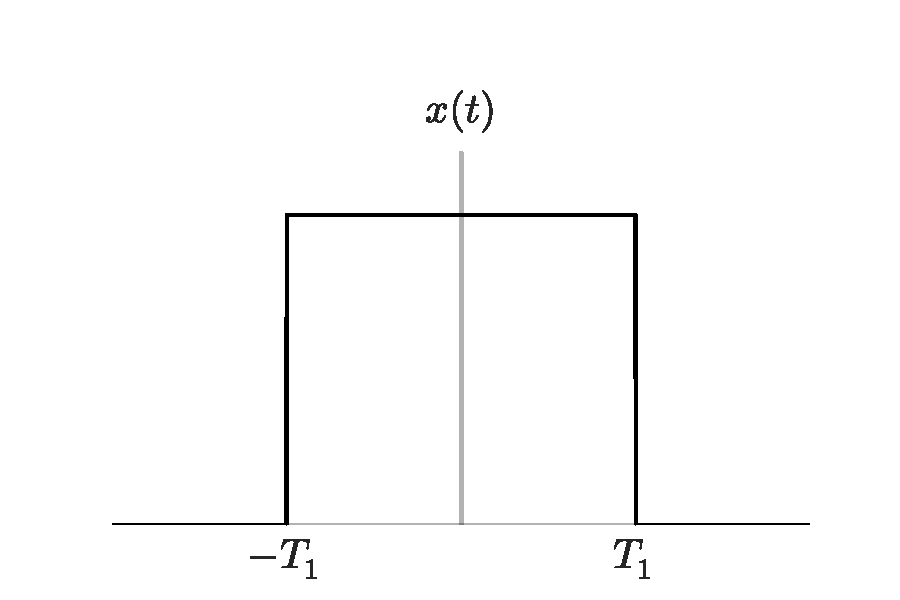
\includegraphics[width=3in]{notes.02.square.pdf}



gives 
\[
X(jw) = \int_{-T_1}^{T_1} e^{-j\omega t} dt = 2 \frac{\sin \omega T_1}{\omega}
\]
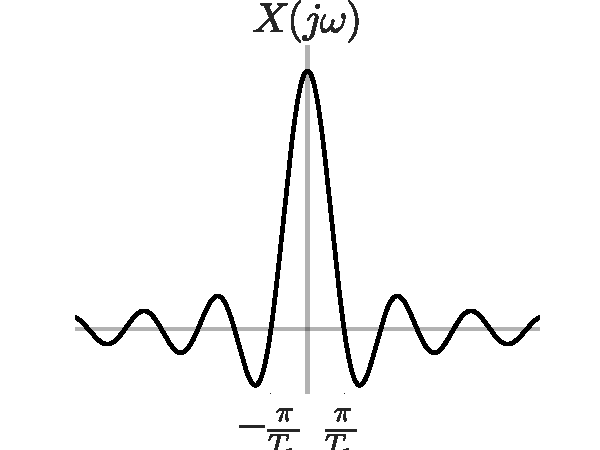
\includegraphics[width=3in]{notes.02.sinc.pdf}


\subsection{Periodic functions}
Consider a signal whose Fourier transform is 
\[
X(j\omega) = 2 \pi \delta(\omega - \omega_0)
\]

we see
\[
x(t) = \frac{1}{2\pi}\int_{-\infty}^{\infty} 2\pi \delta(\omega - \omega_0) e^{j \omega t} d\omega = e^{j\omega_0  t}
\]


Remember that
\[
cos(\omega_0 t) = \frac{e^{j\omega_0 t} + e^{-j\omega_0 t}}{2}
\]

We can use linearity above and arrive at 
\[
\mathscr{F} \{ cos(\omega_0 t) \} = \pi \delta(\omega - \omega_0) + \pi \delta(\omega - \omega_0)
\]


\subsection{Properties}
We start off with 
\[ 
x(t) \ftarrow X(j\omega)
\]
\[ 
y(t) \ftarrow Y(j\omega)
\]

Linearity : 
\[
ax(t) + by(t) \ftarrow aX(j\omega) + bY(j\omega)
\]

Time-shifting: 
\[
x(t - t_0) \ftarrow e^{-j\omega t_0}X(j\omega)
\]

\subsubsection{conjugation and conjugate symmetry}
\subsection{Convolution property}
Consider 
\[
y(t) = \int_{-\infty}^{\infty}x(\tau) h(t-\tau) d\tau
\]
We want $Y(j\omega)$ which is 
\begin{align}
Y(j\omega) &= \mathscr{F} \{ y(t) \} \\
&= \int_{-\infty}^{\infty} \left[ \int_{-\infty}^{\infty}x(\tau) h(t-\tau) d\tau \right]  e^{-j \omega t} dt \\
& = \int_{-\infty}^{\infty} x(\tau) \left[ \int_{-\infty}^{\infty}h(t-\tau) e^{-j\omega t} dt \right]  d\tau && \text{Swap order of integration}\\
& = \int_{-\infty}^{\infty} x(\tau) \left[ H(j\omega) e^{-j\omega \tau} \right] d\tau  && \text{Bracketed term via time-shifting}\\
& = H(j\omega) \int_{-\infty}^{\infty} x(\tau) e^{-j\omega \tau} d\tau \\
& = H(j\omega) X(j\omega) 
\end{align}


And thus we arrive at the celebrated property, 


\[
y(t) = h(t) * x(t) \ftarrow Y(j\omega) = H(j\omega) X(j\omega)  
\]


\subsection{Persaval}
If $x(t)$ and $X(j\omega)$ are a Fourier transform pair, then
\[
\int_{-\infty}^{\infty} | x(t) | ^2 dt = \frac{1}{2\pi} \int_{-\infty}^{\infty} |X(j\omega)| ^2 d\omega
\]

which can be seen via 
\begin{align}
  \int_{-\infty}^{\infty} |x(t)|^2 dt  &= \int_{-\infty}^{\infty} x(t)x^*(t) dt \\
  &= \int_{-\infty}^{\infty} x(t) \left[ \frac{1}{2\pi} \int_{-\infty}^{\infty} X^*(j\omega) e^{-j\omega t} d\omega \right] dt && \text{apply inverse FT} \\
  &=  \frac{1}{2\pi} \int_{-\infty}^{\infty} X^*(j\omega) \left[ \int_{-\infty}^{\infty} x(t) e^{-j\omega t} dt \right] d\omega && \text{Swap order of integration}\\
&= \frac{1}{2\pi} \int_{-\infty}^{\infty} |X(j\omega)| ^2 d\omega && \text{bracket term is FT} \\ 
\end{align}

Thus the total energy in a singal may be found by computing the energy per unit time $|x(t)|^2$ and integrating over all time or computing the energy per unit frequency $|X(j\omega)|^2 / 2\pi$ and integrating over all frequencies. 

\subsection{Duality}
\fxwarning{Do This}

\subsection{Multiplication in the time domain}

We saw that convolution in the time domain corresponds to multiplication in the frequency domain. Because of duality, we expect the dual property to hold -- multiplication in the time domain is equivalent to convolution in the frequency domain. 
\[
r(t) = s(t)p(t) \ftarrow R(j\omega) = \frac{1}{2\pi}[S(j\omega) * P(j\omega)]
\]

Multiplication of one signal by another can be viewed as modulating the amplitude of one
signal by another. 


\section{An introduction to Filtering}
\fxwarning{Give audio example}

\subsection{Bandwidth and Phase}



\section{Magnitude and Phase}

We often write complex numbers as a real part and an imaginary part, 
\[
z = x + j y
\]

but we can also write them in polar form, 
\[
r = |z| = \sqrt{x^2 + y^2}
\]

\[
\phi = \operatorname{arg}(z) = \operatorname{atan2} (y, x)
\]

and then we arrive at $ = r e^{j\phi}$ 


Like all complex-valued functions, we can represent the complex-valued Fourier transform 
in terms of magnitude and phase:

\[
X(j\omega) = |X(j\omega)| e^{j\sphericalangle X(j\omega)}
\]

We think of $|X(j\omega)|^2|$ as the energy in the signal at frequency $\omega$, 
but phase is vital too. For example, from the time reveral property, we 
know that 
\[
x(-t)  \ftarrow X(-j\omega)
\]

so the signals $x(t)$ and $x(-t)$ have the same magnitude fourier transform but 
very different phases! 


\section{The Discrete Fourier Transform}

\[
x[n] = \frac{1}{2\pi}\int_{2\pi} X(e^{jw})e^{j\omega n} d\omega
\]

\[
X(e^{j\omega}) = \sum_{n=-\infty}^{\infty} x[n] e^{-j\omega n}
\]
This looks a lot more like an inner product!

Remember from before : Discrete-time complex expoenntntials that differe in frequency by a multiple of 2pi are identicial. Thus $X(e^{j\omega})$ is periodic with period $2\pi$. 


% %\section{The Fast Fourier Transform}


% \section{Analytic Signals}
% Most signals in the real world are real-valued. 

% Physicsists always say ``Well we can just use a complex signal and
% then take the real part'' but

% 1. Why? 

% 2. Ok, there are a whole bunch of ways to create a complex signal from
% a real one, why do we do it a certain way? 

% 3. I and Q -- quadrature signals

% 4. Negative Frequency


% \section{The Discrete-time Fourier Transform}
% \[
% x[n] = \frac{1}{2\pi} \int_{2\pi} X(e^{j\omega}) e^{j\omega n} d\omega
% \]

% \[
% X(e^{j\omega}) = \sum_{n=-\infty}^{\infty} x[n] e^{-j \omega n}
% \]

% \fxwarning{Why is this so different? Explain it} 


\end{document}
